\documentclass[10pt]{article}

\usepackage[margin=1in]{geometry}
\usepackage[T1]{fontenc}
\usepackage{lmodern}
\usepackage{setspace}
\usepackage{amsmath, amssymb}
\usepackage{tikz}
\usetikzlibrary{shapes}
\usepackage{enumitem}
\usepackage[normalem]{ulem}
\usepackage{float}
\usepackage{xcolor}


\setlength{\parindent}{0pt}
\setlength{\parskip}{0.35em}

\onehalfspacing

\begin{document}

\section*{Chapter 1 Notes}

\subsection*{Statistics Definitions}

\textbf{Global definition:} Statistics involves collecting, organizing, summarizing, presenting, and analyzing data, as well as making inferences, conclusions, and decisions based on data.

\textbf{Statistical definition:} A \underline{statistic} is a numerical value calculated from data (e.g.\ mean, proportion, standard deviation).

\vspace{0.5em}

\textit{Probability vs Statistics:}
\begin{itemize}
    \item \textbf{Probability (deductive):} Population $\rightarrow$ Sample
    \item \textbf{Statistics (inductive):} Sample $\rightarrow$ Population
\end{itemize}

\subsection*{Basic Terminology}
\underline{Individuals}: Objects on which data are collected (people, animals, plots of land, etc.).\\
\underline{Variable}: Any characteristic of an individual.\\
\underline{Population}: The entire group of individuals of interest.\\
\underline{Sample}: A subset of individuals taken from the population.\\
\underline{Statistical Inference}: Drawing conclusions about a population based on a sample.


\subsection*{Sampling Methods}

\underline{Simple Random Sample (SRS):}
\begin{itemize}
  \item Every possible group of size $n$ has an equal chance of being selected.
  \item Helps avoid bias in sampling.
  \item Can be selected using random number tables or software.
\end{itemize}

\underline{Stratified Random Sampling:}
\begin{itemize}
  \item The population is divided into \underline{homogeneous groups} 
        \textit{(individuals are similar with respect to the variable being studied)} 
        called \underline{strata}.
  \item A simple random sample is taken from each \underline{stratum}. 
        \textit{(one subgroup of the population created)}
  \item Ensures that important subgroups are neither over nor under represented.
\end{itemize}

\subsection*{Types of Variables}

\underline{Categorical Variable}: Places individuals into categories (e.g.\ gender, major). These are qualitative.

\underline{Quantitative Variable}: Takes numerical values for which arithmetic operations are meaningful.

\begin{itemize}
    \item \underline{Discrete}
    \item \underline{Continuous}
\end{itemize}


\subsection*{Distributions}

\underline{Distribution}: Describes what values a variable takes and how often those values occur.
When examining a distribution, look for:
\begin{itemize}
    \item \textbf{Shape}
    \item \textbf{Center}
    \item \textbf{Spread}
    \item \textbf{Outliers}
\end{itemize}
\underline{Outlier}: An individual value that falls outside the overall pattern of the data.

\subsection*{Describing Distributions with Numbers}

\underline{Central Tendency}: Describes where the data cluster or center.
\begin{itemize}
    \item \underline{Mean}: average value
    \item \underline{Median}: middle value
\end{itemize}

The mean is more sensitive to extreme values than the median.

Changing a single data value will always change the mean, but may not change the median.

If a distribution is exactly symmetric, the mean and median are equal.

\underline{Trimmed Mean}: The mean computed after removing extreme values. It is more resistant to outliers than the mean but uses more information than the median.

\subsection*{Measures of Spread}

\underline{Range}: Maximum minus minimum (very sensitive to extreme values).

\underline{Sample Variance}:
\[
\boxed{
s^2 = \frac{1}{n-1} \sum_{i=1}^{n} (x_i - \bar{x})^2
}
\]

\underline{Standard Deviation}:
\[
\boxed{
s = \sqrt{s^2}
}
\]

\underline{Degrees of Freedom}: The number of independent pieces of information available to estimate variability.

\section*{Chapter 2, Jan 9th}

\underline{Experiment}: A process that generates an outcome.

\vspace{0.5em}

\underline{Sample Space ($S$)}: The set of all possible outcomes of an experiment.

\vspace{1em}

\textbf{Example 1:}

Select 3 items from a production line. Each item can be classified as either defective ($D$) or non-defective ($N$).

\[
S = \{ DDD, DDN, DND, NDD, DNN, NDN, NND, NNN \}
\]

Since each item has 2 possible outcomes,
\[
|S| = 2^3 = 8
\]

\vspace{1em}

\textbf{Example 2:}

\[
S = \{ (x,y) \mid x^2 + y^2 \le 4 \}
\]

\vspace{1em}

\underline{Event ($A$)}: A subset of the sample space $S$.

\vspace{0.5em}

\textbf{Examples of events:}
\[
A = \{ DDD, DDN, DND, NDD \}
\]
\[
B = \{ NNN \}
\]
\[
C = \{ (x,y) \mid x^2 + y^2 \le 4 \}
\]

\vspace{1em}

\underline{Event Operations}:
\begin{itemize}
  \item \underline{Complement}: $A^c$ (or $A'$)
  \item \underline{Intersection}: $A \cap B$
  \item \underline{Union}: $A \cup B$
  \item \underline{Null Event}: $\varnothing$
\end{itemize}

If
\[
A \cap B = \varnothing,
\]
then $A$ and $B$ are \underline{mutually exclusive}.

\vspace{1em}

\textbf{Example (Venn Diagram):}

\begin{center}
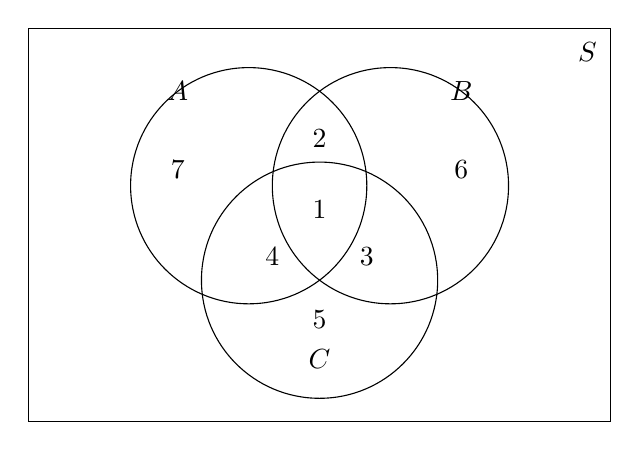
\begin{tikzpicture}[scale=1]

% Sample space
\draw (-2.8,-3) rectangle (4.6,2);

% Circles
\draw (0,0) circle (1.5);        % A
\draw (1.8,0) circle (1.5);      % B
\draw (0.9,-1.2) circle (1.5);   % C

% Labels
\node at (-0.9,1.2) {$A$};
\node at (2.7,1.2) {$B$};
\node at (0.9,-2.2) {$C$};
\node at (4.3,1.7) {$S$};

% Region numbers
\node at (-0.9,0.2) {7};        % A only
\node at (0.9,0.6) {2};         % A ∩ B
\node at (2.7,0.2) {6};         % B only
\node at (0.3,-0.9) {4};        % A ∩ C
\node at (1.5,-0.9) {3};        % B ∩ C
\node at (0.9,-0.3) {1};        % A ∩ B ∩ C
\node at (0.9,-1.7) {5};        % C only

\end{tikzpicture}
\end{center}

\[
A = \{ DDD, DDN, DND, NDD \}, \quad
B = \{ NNN \}
\]

\[
A \cup B = \{ DDD, DDN, DND, NDD, NNN \}
\]

\[
A \cap B = \varnothing
\]

Jan 12th 
\section*{Chapter 2: January 12}

\subsection*{Review}
{\itshape

\begin{enumerate}
    \item \underline{Experiment}: A process that generates an outcome.
    
    \item \underline{Sample Space} ($S$): The set of all possible outcomes of an experiment.
    
    \item \underline{Event Operations}:
    \begin{itemize}
        \item Complement: $A' \; (A^c)$
        \item Intersection: $A \cap B$
        \item Union: $A \cup B$
        \item Null Event: $\varnothing$
    \end{itemize}
    
    \item If $A \cap B = \varnothing$, then $A$ and $B$ are called \underline{mutually exclusive}.
\end{enumerate}

\fbox{
\parbox{0.95\textwidth}{
\[
(A \cap B)' = A' \cup B'
\]
\[
(A \cup B)' = A' \cap B'
\]
\[
A \cap \varnothing = \varnothing
\]
\[
A \cup \varnothing = A
\]
\[
A \cap (B \cup C) = (A \cap B) \cup (A \cap C)
\]
}}
}

\subsection*{Probability}

$P(A)$ = probability of event $A$: the proportion of times the event occurs in infinitely many repetitions of the experiment.

\medskip

\textcolor{blue}{\textbf{Theorem2.1:}}
\[
0 \le P(A) \le 1
\]

\medskip

\fbox{
\parbox{0.95\textwidth}{
\[
P(A) + P(A') = 1
\]

\[
P(A \cup B) = P(A) + P(B) - P(A \cap B)
\]

\[
\begin{aligned}
P(A \cup B \cup C) =\;& P(A) + P(B) + P(C) \\
&- P(A \cap B) - P(A \cap C) - P(B \cap C) \\
&+ P(A \cap B \cap C)
\end{aligned}
\]
}}

\medskip

\subsection*{Mutually Exclusive Events}

\underline{Definition}:  
If $A_1, A_2, \ldots, A_n$ are mutually exclusive, then
\[
P(A_1 \cup A_2 \cup \cdots \cup A_n)
=
P(A_1) + P(A_2) + \cdots + P(A_n)
\]

If
\[
A_1 \cup A_2 \cup \cdots \cup A_n = S,
\]
then $\{A_1, A_2, \ldots, A_n\}$ is a \underline{partition} of $S$.

\medskip
\begin{figure}[H]
\centering
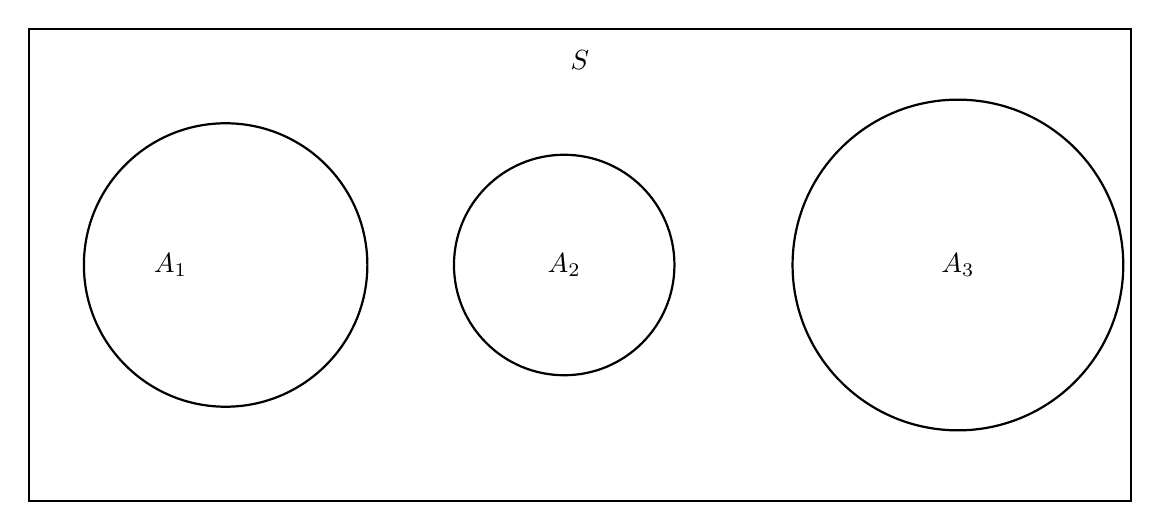
\begin{tikzpicture}[scale=1]

% Sample space
\draw[thick] (0,0) rectangle (14,6);
\node at (7,5.6) {$S$};

% A1
\draw[thick] (2.5,3) circle (1.8);
\node at (1.8,3) {$A_1$};

% A2
\draw[thick] (6.8,3) circle (1.4);
\node at (6.8,3) {$A_2$};

% A3
\draw[thick] (11.8,3) circle (2.1);
\node at (11.8,3) {$A_3$};

\end{tikzpicture}
\caption{Partition of the sample space $S$ into $A_1, A_2, A_3$}
\end{figure}


\subsection*{Example}

In a class of 33 students:
\begin{itemize}
    \item 17 earned an A on the midterm
    \item 14 earned an A on the final
    \item 11 earned no A on either exam
\end{itemize}

Find the probability that a randomly selected student earned A's on \underline{both} exams.

\begin{figure}[H]
\centering
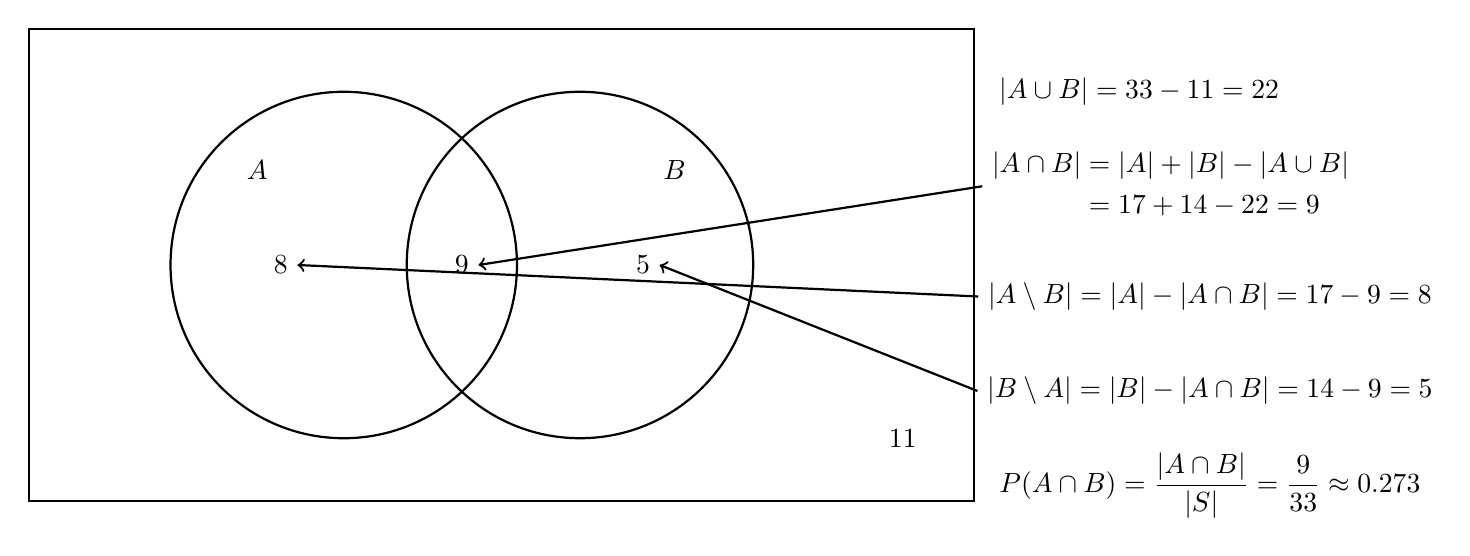
\begin{tikzpicture}[scale=1]

% -------------------------
% Sample space
% -------------------------
\draw[thick] (0,0) rectangle (12,6);

% -------------------------
% Circles A and B
% -------------------------
\draw[thick] (4,3) circle (2.2);
\draw[thick] (7,3) circle (2.2);

\node at (2.9,4.2) {$A$};
\node at (8.2,4.2) {$B$};

% -------------------------
% Region numbers
% -------------------------
\node (Aonly) at (3.2,3.0) {$8$};
\node (AB)    at (5.5,3.0) {$9$};
\node (Bonly) at (7.8,3.0) {$5$};
\node (outside) at (11.1,0.8) {$11$};

% -------------------------
% Calculation text blocks
% -------------------------
\node[align=left] (calcUnion) at (14.1 ,5.2) {$|A \cup B| = 33 - 11 = 22$};

\node[align=left] (calcInter) at (14.5,4.0) {$\begin{aligned}
|A \cap B|
&= |A| + |B| - |A \cup B| \\
&= 17 + 14 - 22 = 9
\end{aligned}$};

\node[align=left] (calcAonly) at (15,2.6) {$|A \setminus B| = |A| - |A \cap B| = 17 - 9 = 8$};

\node[align=left] (calcBonly) at (15,1.4) {$|B \setminus A| = |B| - |A \cap B| = 14 - 9 = 5$};

\node[align=left] (calcProb) at (15 ,0.2) {$P(A \cap B)=\dfrac{|A \cap B|}{|S|}=\dfrac{9}{33}\approx 0.273$};

% -------------------------
% Arrows pointing to regions
% -------------------------
\draw[->, thick] (calcInter.west) -- (AB.east);
\draw[->, thick] (calcAonly.west) -- (Aonly.east);
\draw[->, thick] (calcBonly.west) -- (Bonly.east);

\end{tikzpicture}
\caption{Events $A$: A on midterm, $B$: A on final, with region counts and calculations}
\end{figure}

\textcolor{blue}{\textbf{Theorem 2.2 (Equally Likely Outcomes):}}  

If the sample space $S$ has a finite number of outcomes and all outcomes are equally likely, then for any event $A$,
\[
P(A) = \frac{|A|}{|S|}
\]

where  \\
\text{A: the event of interest (a subset of the sample space $S$),}\\
\text{S: the sample space, i.e.\ the set of all possible outcomes.}


\subsection*{Example 1: Poker Hands Basics}

A standard deck has:
\[
4 \text{ suits} \times 13 \text{ denominations (A,2,3,\ldots,Q,K)} = 52 \text{ cards}.
\]

A poker hand consists of 5 cards chosen from 52:
\[
|S| = \binom{52}{5} = 2,\!598,\!960.
\]

\subsection*{Combinations Reminder}

If there are 3 objects $\{A,B,C\}$ and we choose 2:
\[
\binom{3}{2} = \frac{3!}{(3-2)!2!}.
\]

Order does \underline{not} matter.

\subsection*{Example 2: Probability of 2 Aces and 1 Jack}

A 5-card hand contains:
\begin{itemize}
    \item exactly 2 aces,
    \item exactly 1 jack,
    \item 2 cards that are neither aces nor jacks.
\end{itemize}


\[
P(\text{2 aces and 1 jack})
=
\frac{\binom{4}{2}\binom{4}{1}\binom{44}{2}}{\binom{52}{5}}.
\]

\subsection*{Example 3: Probability of a Full House}

A full house consists of:
\begin{itemize}
    \item 3 cards of one denomination
    \item 2 cards of a different denomination
\end{itemize}

Number of full house hands:
\[
\binom{13}{1} \binom{4}{3}
\binom{12}{1} \binom{4}{2}.
\]

Thus,
\[
P(\text{full house})
=
\frac{\binom{13}{1}\binom{4}{3}\binom{12}{1}\binom{4}{2}}{\binom{52}{5}}.
\]

\subsection*{Example 4: Probability of Four of a Kind}

A four of a kind consists of:
\begin{itemize}
    \item 4 cards of the same denomination
    \item 1 remaining card of a different denomination
\end{itemize}

Number of such hands:
\[
\binom{13}{1}\binom{4}{4}\binom{48}{1}.
\]

Thus,
\[
P(\text{four of a kind})
=
\frac{\binom{13}{1}\binom{4}{4}\binom{48}{1}}{\binom{52}{5}}.
\]


\subsection*{Example 5: Probability of Exactly One Pair}

An \textbf{excatly} one-pair hand consists of:
\begin{itemize}
    \item 1 pair
    \item 3 cards of different denominations, none matching the pair
\end{itemize}

Number of such hands:
\[
\binom{13}{1}\binom{4}{2}
\binom{12}{3}\binom{4}{1}^3.
\]

Thus,
\[
P(\text{exactly one pair})
=
\frac{
\binom{13}{1}\binom{4}{2}
\binom{12}{3}\binom{4}{1}^3
}{
\binom{52}{5}
}.
\]

\subsection*{Note*: Counting Patterns }

\[
\binom{a}{b}
\]

\textbf{Meaning:} Choose b different items from $a$ \textbf{at once}, order does not matter.

\textbf{Key features:}
\begin{itemize}
    \item No repeats
    \item Grouped choice
    \item Used when items must be \underline{distinct}
\end{itemize}

\vspace{0.5em}

\[
\binom{a}{1}^b
\]

\textbf{Meaning:} Make $b$ \underline{independent choices}, each time choosing 1 item from $c$.

\textbf{Key features:}
\begin{itemize}
    \item Repeats allowed
    \item Choices are independent
    \item Used when selections do \underline{not} restrict each other
\end{itemize}

\vspace{0.5em}

\noindent
\textcolor{red}{\textbf{Rule to Remember:}}

\[
\textcolor{red}{\text{Different items, no repeats } \Rightarrow \binom{a}{b}}
\]

\[
\textcolor{red}{\text{Independent choices } \Rightarrow \binom{c}{1}^b}
\]



\end{document}
